\documentclass[../main]{subfiles}
\begin{document}

\chapter{Vectores en R$^n$}
En este apartado se detallan sobre los vectores, un concepto fundamental para el estudio del cálculo de funciones de varias variables. \\[0.2cm]
\textbf{Definición:} Los vectores son objetos matemáticos que tienen módulo, dirección y sentido. Se puede representar gráficamente a cualquier vector mediante una flecha.
\begin{figure}[h!]
    \centering
    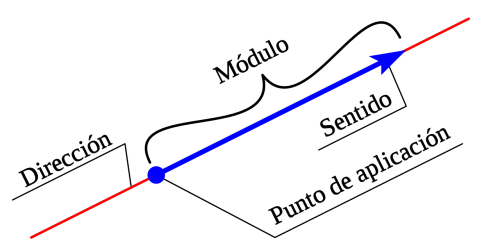
\includegraphics[scale=0.7]{Cálculo/CÁLCULO VECTORIAL/images/img1.png}
    \caption{Componentes de un vector}
    \label{fig:my_label}
\end{figure}

Un vector en $\mathbb{R}^3$ es una terna ordenada de números reales, y se denota de la siguiente forma:
\begin{equation}
    \Vec{u}=(x,y,z)
\end{equation}
Y de manera general para un vector en $\mathbb{R}^n$ primero se define el espacio vectorial $\mathbb{R}^n$ el cual se denota como el conjunto de las n-tuplas ordenadas de números reales, así $\mathbb{R}^n:(x_1,x_2,x_3,\cdots,x_n)$ donde $x_i \in \mathbb{R}$, $1\leq i \leq n$. Los elementos de $\mathbb{R}^n$ también se suelen denominar vectores de orden $n$.
\begin{itemize}
    \item \textbf{Ejemplo de Vector en $\mathbb{R}^n:$}
        \begin{equation}
            \Vec{u}=(u_1,u_2,u_3,\cdots, u_n)
        \end{equation}
\end{itemize}
\section{Norma de un Vector}
La norma o \textit{longitud} de un vector $\Vec{u}=(u_1,u_2,\cdots, u_n)$, esta definida como:
\begin{equation}
    |\Vec{u}|=\sqrt{u_1^2+u_2^2+\cdots u_n^2}
\end{equation}
\section{Distancia entre dos puntos}
Sean $\Vec{u}=(u_1,u_2,\cdots, u_n)$ y $\Vec{v}=(v_1,v_2,\cdots, v_n)$ en $\mathbb{R}^n$, se define el producto punto o escalar como:
\begin{equation}
    \Vec{u} \cdot \Vec{v}=u_1 v_1+ u_2 v_2 +\cdots +u_n v_n=\sum_{i=1}^n u_i v_i
\end{equation}
\section{Producto Cruz o Vectorial}
Teniendo los vectores $\Vec{u}=(u_1,u_2,\cdots, u_n)$ y $\Vec{v}=(v_1,v_2,\cdots, v_n)$ se define el producto vectorial de dos vectores en $\mathbb{R}^3$ como:
\begin{equation}
    \vec{u} \times \vec{v}=\left |
    \begin{matrix}
    \hat{i} & \hat{j} & \hat{k} \\
    u_1     & u_2     & u_3 \\
    v_1     & v_2     & v_3
    \end{matrix}
    \right|
\end{equation}
\chapter{Funciones vectoriales de una variable real}
Aquí nos referimos a aquellas funciones vectoriales las cuales tienen su dominio en un subconjunto de $\mathbb{R}$ y un contradominio en un espacio vectorial $\mathbb{R}^n$. \\[0.2cm]
De este modo una función vectorial $f$ asocia a cada elemento $t$ de un conjunto $\mathbb{D}$ de números reales, un único vector $f(t)$.
\begin{align}
f:\mathbb{D} & \subseteq \mathbb{R} \rightarrow \mathbb{R}^n \nonumber \\
t & \rightarrow f(t) \nonumber \\
f(t) = [ x_1 (t) &, x_2 (t), \ldots , x_n (t) ] \in \mathbb{R}^n \nonumber
\end{align}
\chapter{Dominio de una función vectorial}
El dominio de una función vectorial $f(t)$ esta referido a aquellos valores permitidos por $t$.\\[0.2cm]
Si $f(t)$ esta definida en términos de las funciones de las componentes y no esta especificada explícitamente el dominio, entonces se entiende que el dominio es la intersección de los dominios naturales de las funciones de las componentes, por lo que este recibe el nombre de dominio natural de $f(t)$:
\begin{equation}
    f(t)=(x_1(t),x_2(t),\ldots,x_n(t)) \in \mathbb{R}^n
\end{equation}
Entonces su dominio es:
\begin{equation}
    Dom(f)=\bigcap_{i=1}^n Dom(x_i(t))
\end{equation}
\chapter{Limite y continuidad de una función vectorial}
El límite de una función vectorial $f$ se define tomando los límites de sus funciones componentes: 
Si $f(t)=(x_1(t),x_2(t),\ldots,x_n(t)$, entonces
\begin{equation}
    \lim_{t \rightarrow a}=\left ( \lim_{t \rightarrow a} x_1(t), \lim_{t \rightarrow a} x_2(t),\ldots, \lim_{t \rightarrow a} x_n(t) \right)
\end{equation}
Siempre y cuando los límites de las funciones componentes existan.\\[0.2cm]
También se tiene que una función vectorial $f$ será continua si se cumple que:
\begin{equation}
    \lim_{t \rightarrow a} f(t)=f(a)
\end{equation}
\chapter{Funciones vectoriales y curvas en el espacio}
Existe una estrecha relación entre las funciones vectoriales continuas y las curvas en el espacio. Supongase que $x_1$, $x_2$ y $x_3$ son funciones continuas con valores reales en un intervalo \textit{I}. Entonces el conjunto $\mathbb{C}$ de todos los puntos $(x,y,z)$ en el espacio, donde:
\begin{equation}
    x=x_1(t), \qquad y=x_2(t), \qquad z=x_3(t)
\end{equation}
Las ecuaciones anteriores se llaman \textbf{ecuaciones paramétricas} de $\mathbb{C}$ y $t$ se llama \textbf{parámetro}. Si consideramos ahora la función vectorial:
\begin{equation}
    \mathbf{r}(t)=\langle x_1(t),x_2(t),x_3(t)\rangle
\end{equation}
Entonces $\mathbf{r}(t)$ es el vector de posición del punto $P(x_1(t),x_2(t),x_3(t))$ en $\mathbb{C}$. Así, toda función vectorial continua $\mathbf{r}$ define una curva en el espacio $\mathbb{C}$ trazada por la punta del vector en movimiento $\mathbf{r}(t)$.
\chapter{Derivadas e integrales de funciones vectoriales}
\section{Derivadas}
La derivada $\mathbf{r}^{\prime}$ de una función vectorial $\mathbf{r}$ se define casi de la misma manera que las funciones con valores reales:
\begin{equation}
    \dfrac{d\mathbf{r}}{dt}=\mathbf{r}^{\prime}(t)=\lim_{h\rightarrow 0} \dfrac{\mathbf{r}(t+h)-\mathbf{r}(t)}{h}
\end{equation}
De aqui se tiene que cuando $h \rightarrow 0$, parece que este vector se aproxima a un vector que está en la recta tangente. Por esta razón, el vector $\mathbf{r}^{\prime}(t)$ se llama vector tangente a la curva definida por $\mathbf{r}$ en el punto $P$, siempre y cuando $\mathbf{r}^{\prime}(t)$ exista y $\mathbf{r}^{\prime}(t)\neq 0$. La recta tangente a $\mathbb{C}$ en $P$ se define como la recta que pasa por $P$ paralela al vector tangente $\mathbf{r}^{\prime}(t)$. Mencionando el vector tangente unitario, el cual es:
\begin{equation}
    \mathbf{T}(t)=\dfrac{\mathbf{r}^{\prime}(t)}{|\mathbf{r}^{\prime}(t)|}
\end{equation}
\textbf{Teorema:} Si $\mathbf{r}(t)=\langle x_1(t),x_2(t),x_3(t) \rangle=x_1(t)\hat{i}+x_2(t)\hat{j}+x_3(t)\hat{k}$, donde $x_1$,$x_2$ y $x_3$ son funciones derivables, entonces:
\begin{equation}
    \mathbf{r}^{\prime}=\langle x_1^{\prime}(t),x_2^{\prime}(t),x_3^{\prime}(t) \rangle=x_1^{\prime}(t)\hat{i}+x_2^{\prime}(t)\hat{j}+x_3^{\prime}(t)\hat{k}
\end{equation}
\section{Integrales}
La integral definida de una función vectorial continua $\mathbf{r}(t)$ puede definirse casi de igual forma que las funciones con valores salvo que la integral es un vector. Y se puede expresar la integral de $\mathbf{r}$ en términos de las integrales de sus funciones componentes $x_1$,$x_2$ y $x_3$ como sigue:
\begin{align}
   \int_a^b \mathbf{r}(t)dt & = \lim_{n \rightarrow \infty} \sum_{i=1}^n \mathbf{r}(t_i^{*})\Delta t \nonumber \\
   \int_a^b \mathbf{r}(t)dt & = \lim_{n\rightarrow \infty} \left[ \left( \sum_{i=1}^n x_1(t_i^{\*})\Delta t \right)\hat{i}+\left( \sum_{i=1}^n x_2(t_i^{\*})\Delta t \right)\hat{j}+\left( \sum_{i=1}^n x_3(t_i^{\*})\Delta t \right)\hat{k} \right]
\end{align}
Quedando así:
\begin{align}
    \int_a^b \mathbf{r}(t)dt=\left( \int_a^b x_1(t)dt \right)\hat{i}+\left( \int_a^b x_2(t)dt \right)\hat{j}+\left( \int_a^b x_3(t)dt \right)\hat{k}
\end{align}
Extendiendo el teorema fundamental del cálculo a las funciones vectoriales continuas como sigue:
\begin{align}
    \int_a^b \mathbf{r}(t)dt=\mathbf{R}(t)]\_{a}^b =\mathbf{R}(b)-\mathbf{R}(a)
\end{align}
donde $\mathbf{R}$ es una antiderivada de $\mathbf{r}$, es decir $\mathbf{R}^{\prime}(t)=\mathbf{r}(t)$.
\chapter{Longitud de arco y curvatura}
\section{Longitud de arco}
Supóngase que la curva tiene la ecuación vectorial 
$$\mathbf{r}(t)=\langle x_1(t),x_2(t),x_3(t) \rangle$$
donde $a\leq t \leq b$ o de igual manera las ecuaciones paramétricas $x=x_1(t)$, $y=x_2(t)$ y $z=x_3(t)$, donde $x_1^{\prime}$,$x_2^{\prime}$ y $x_3^{\prime}$ son continuas. Si la curva es recorrida exactamente una vez cuando $t$ se incrementa de $a$ a $b$, es posible demostrar que su longitud es:
\begin{align}
    L&=\int_a^b \sqrt{[x_1^{\prime}]^2+[x_2^{\prime}]^2+[x_3^{\prime}]^2} dt \\
   L&=\int_a^b \sqrt{\left(\dfrac{dx}{dt} \right)^2+\left(\dfrac{dy}{dt} \right)^2+\left(\dfrac{dz}{dt} \right)^2} dt
\end{align}
De forma más compacta:
\begin{align}
    L=\int_a^b |\mathbf{r}^{\prime}(t)|dt
\end{align}
\section{Curvatura}
La curvatura de $\mathbb{C}$ en un punto dado es una medida de lo rápido que la curva cambia de dirección en ese punto. Más específicamente se define como la magnitud de la razón de cambio del vector tangente unitario con respecto a la longitud de arco.\\[0.2cm]
\textbf{Definición:} La curvatura de una curva es: 
\begin{equation}
    \kappa=\left | \dfrac{d\mathbf{T}}{ds} \right |=\dfrac{|\mathbf{T}^{\prime}(t)|}{\mathbf{r}^{\prime}(t)|}
\end{equation}

\textbf{Teorema:} La curvatura de la curva dada por la función vectorial $\mathbf{r}$ es: 
\begin{equation}
    \kappa=\dfrac{|\mathbf{r}^{\prime}(t)\times \mathbf{r}^{''}(t)|}{|\mathbf{r}^{'}(t)|^3}
\end{equation}
\end{document}